\section{Ingredienti per Jianico \#2 Stufato di
Almiraj}\label{ingredienti-per-jianico-2-stufato-di-almiraj}

Creature Coinvolte: Aboleth Data Sessione: February 23, 2024 Giocatori
Coinvolti: Bohr Ra, Durso, Gario Miordano Luoghi: Azura, Drakonia
Master: Lorenzo NPC coinvolti: Chef Jianico, Sithau

\href{Durso\%201300f1f2704341b8af557e877374018c.md}{Durso} ,
\href{Bohr\%20Ra\%2064449ef6c46549e9abf62b9d7e01a69d.md}{Bohr Ra} e
\href{Gario\%20Miordano\%20e4415ce5ce8d4e8a834479901942d838.md}{Gario
Miordano} sono convocati da
\href{Sitahu\%203e1abded771c4c39a375ae0243478a44.md}{Sitahu} nel suo
ufficio. Appena varcano la soglia, trovano lo chef Jianico, celebre
maestro culinario di Azura, seduto accanto al quartiermastro. Sithau li
fa accomodare e poi cede la parola allo chef, il quale spiega di essere
stato incaricato da un influente individuo della città di preparare una
cena a base di Almiraj, una prelibatezza culinaria dal gusto sopraffino.
Tuttavia, questo animale prelibato non è reperibile nei territori di
Azura, né tantomeno nei dintorni. Sithau fa entrare quindi nel suo
ufficio lo zoologo della gilda, tale William Sparkle, carico di libri e
pergamene, pronto a delucidare i protettori su ogni aspetto riguardante
l'Almiraj. Sparkle descrive l'Almiraj come un coniglio dotato di un
singolare corno sulla fronte, una creatura estranea alla regione di
Azura ma presente nei territori attualmente occupati dal regno di
\href{Drakonia\%207646694c0d12453293a9b7e41d5cdb15.md}{Drakonia} , un
luogo avvolto nell'oscurità governato da un potente lich, i cui confini
sono presidiati da un'armata di non-morti. Dopo un secolo di isolamento
causato dalla grande guerra, il regno di Drakonia e le terre libere di
Valtara non hanno più avuto contatti. Ai protettori è strettamente
vietato oltrepassare i confini del regno, poiché ciò potrebbe
riaccendere le fiamme della guerra. Fortunatamente, spiega Sparkle,
durante questo periodo dell'anno gli Almiraj risalgono il corso del
fiume Kratos, che sfocia nei territori di Drakonia, arrivando fino a un
boschetto in una radura appena al di là dei confini del regno, dove si
accoppiano. William chiede il motivo di tanto interesse verso questi
magnifici animali, ma riceve solo silenzio come risposta. Insistendo,
diventa sempre più preoccupato di fronte al silenzio imbarazzante e alla
presenza del rinomato chef di Azura. Quando comincia a comprendere la
situazione, tenta di protestare ma viene prontamente interrotto da
Sithau e allontanato dall'ufficio. Sithau torna dai suoi ospiti,
rassicurando lo chef riguardo ai tempi (il boschetto indicato dallo
zoologo dista sei giorni di viaggio a cavallo) e poi provvede a fornire
ai protettori una carrozza trainata da due cavalli, dotata di gabbie
sufficienti per contenere più di dieci conigli. Lo chef ha infatti
bisogno di almeno dieci conigli vivi, poiché sei giorni di viaggio
sarebbero fatali per conigli morti, destinati a decomposizione.

I protettori partono e raggiungono senza intoppi il luogo indicato dallo
zoologo. Esplorano il boschetto ma non trovano alcuna traccia degli
Almiraj. Tuttavia, notano una imponente fortezza sul fiume a poche
centinaia di metri da loro, che funge anche da ponte. Realizzano che
quest ponte-fortezza segna il confine del regno di Drakonia, essendo
presidiata da alcuni soldati. All'improvviso, avvistano un coniglio. Non
riescono a catturarlo ma decidono di seguirlo, finendo davanti al
ponte-fortezza. Capiscono rapidamente che i conigli hanno scelto la
fortezza come rifugio e devono operare con cautela se vogliono
catturarne il maggior numero possibile senza destare sospetti tra le
guardie.

\begin{figure}
\centering
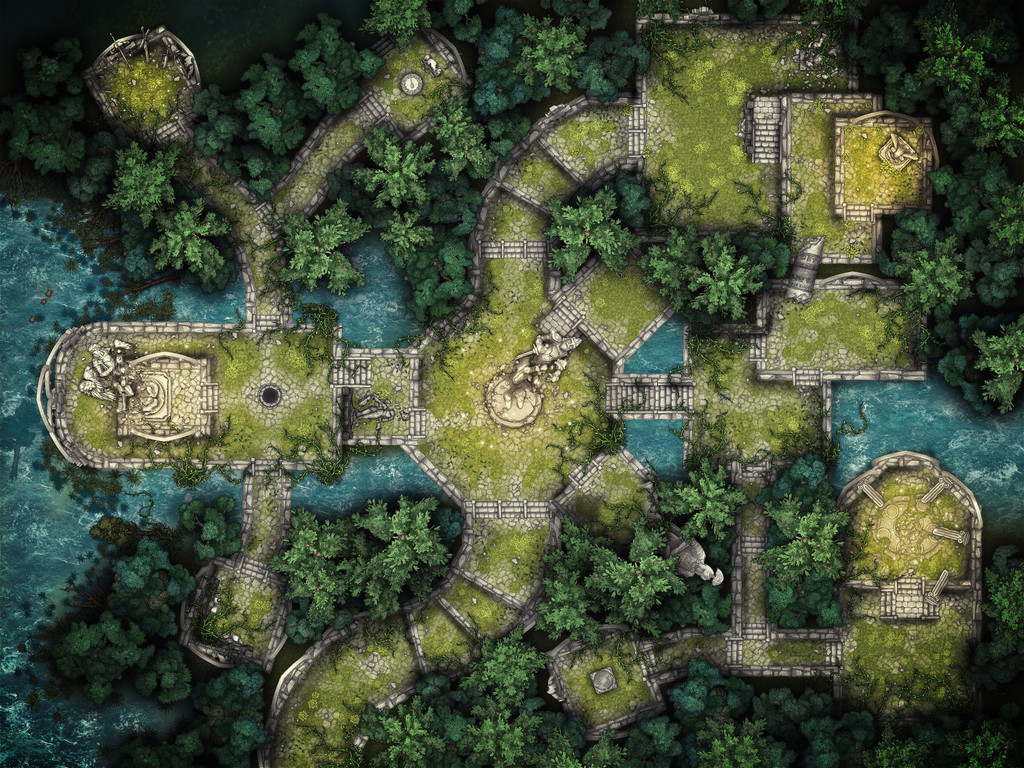
\includegraphics{Ponte-fortezza.jpg}
\caption{Ponte-fortezza.jpg}
\end{figure}

Durso riesce subito a catturare un paio di conigli, mentre Bohr, resosi
invisibile, ne acchiappa un terzo. Durso decide di portare i tre conigli
alla carrozza per imprigionarli nelle gabbie, mentre gli altri
protettori elaborano un piano. Osservando il ponte-fortezza, notano che
è pieno di soldati e che i conigli si muovono tra di loro indisturbati.
È impossibile avvicinarsi ad altri conigli con le guardie così vicine.
Al ritorno di Durso, il piano è pronto: i protettori decidono di
aspettare la notte per agire nell'oscurità e catturare i conigli nelle
loro tane individuate sul ponte-fortezza. Per tutte le ore che i
protettori hanno aspettato fino all'arrivo della notte, i soldati non si
sono mossi, continuando a pattugliare il ponte-fortezza in modo quasi
meccanico e innaturale, senza dare spazio all'azione dei protettori.

I protettori decidono di entrare comunque in azione. Attraggono un
soldato facendo rumore e lo sconfiggono con una serie di attacchi
combinati, scoprendo che sotto l'elmo e l'armatura si cela uno
scheletro, indicando che tutti i soldati sono non-morti. Durso decide di
spogliare il suo avversario e indossare la sua armatura per infiltrarsi
tra i nemici. Borh segue invisibile Durso, fungendo da messaggero tra
lui, travestito tra i nemici, e Gario, nascosto tra i cespugli
all'entrata nord del ponte-fortezza. Durso trova un pozzo chiuso da una
grata e capisce che se riuscisse a rimuoverla, potrebbe gettarvi dentro
più nemici possibile. Propone quindi un piano: mentre Gario distrae i
soldati con del rumore, Borh, invisibile, sposta la grata per rendere il
pozzo accessibile. Il piano viene messo in atto con successo: Bohr apre
la grata, attirando quasi tutti i soldati al pozzo, dopodichè Gario
genera un rumore di urla umane nel fiume, attirando al parapetto del
ponte-fortezza quasi tutti i soldati che scrutavano il pozzo. Durso è
rimasto ora solo con un solo soldato davanti al pozzo. Durso riesce a
eliminare il suo avversario e a farlo precipitare nel pozzo senza farsi
notare dagli altri soldati, tornati alle loro posizioni.
Successivamente, Durso e Borh individuano un luogo sul ponte-fortezza
dove quattro conigli riposano. Decidono di attuare lo stesso piano per
catturarli. Tuttavia, la distrazione di Gario arriva troppo tardi e i
soldati sentono prima gli striduli lamenti dei conigli catturati dai
protettori. Durso decide di continuare a fingere come se niente fosse,
riuscendo a passare inosservato tra i soldati che lo raggiungono, ma
Borh, non avendo via di fuga né più l'invisibilità e con due conigli
agitati nel suo sacco, decide di lanciarsi dalle mura del ponte-fortezza
sugli alberi vicini. Il salto non è impeccabile e Borh, cadendo,
fracassa la testa dei due conigli, ma riesce a non essere notato dai
soldati. Mentre Borh cerca di arrampicarsi tra gli alberi per tornare
sul ponte-fortezza, Durso continua indisturbato a fingere di essere una
sentinella tra i nemici. Tuttavia, quando un soldato nemico, per tornare
alla propria posizione, si trova tra Durso e il pozzo, quest'ultimo non
resiste, e lo spinge nel pozzo sotto gli occhi degli altri soldati, che
partono subito all'inseguimento. Durso fugge verso Gario, mentre Borh,
risalito sul ponte-fortezza, insegue i soldati che inseguono Durso. Ne
scaturisce un combattimento che vede Borh emergere vittorioso,
sconfiggendo i suoi nemici fulminandoli.

Solo un nemico riesce a sfuggire ai protettori, riuscendo a suonare un
corno. Borh nota che dopo il suono del corno, tutte le altre guardie sul
ponte-fortezza fuggono, lasciando la fortezza vuota. Senza comprendere
completamente cosa stia accadendo, i protettori decidono di sfruttare
l'occasione e cercare di catturare più conigli possibile. Tuttavia,
mentre si addentrano nel forte alla ricerca di prede, l'acqua del fiume
che scorre sotto al ponte-fortezza inizia a gonfiarsi: un enorme Aboleth
esce dall'acqua, abbattendosi su di loro. Inizia uno scontro brutale.

\begin{figure}
\centering
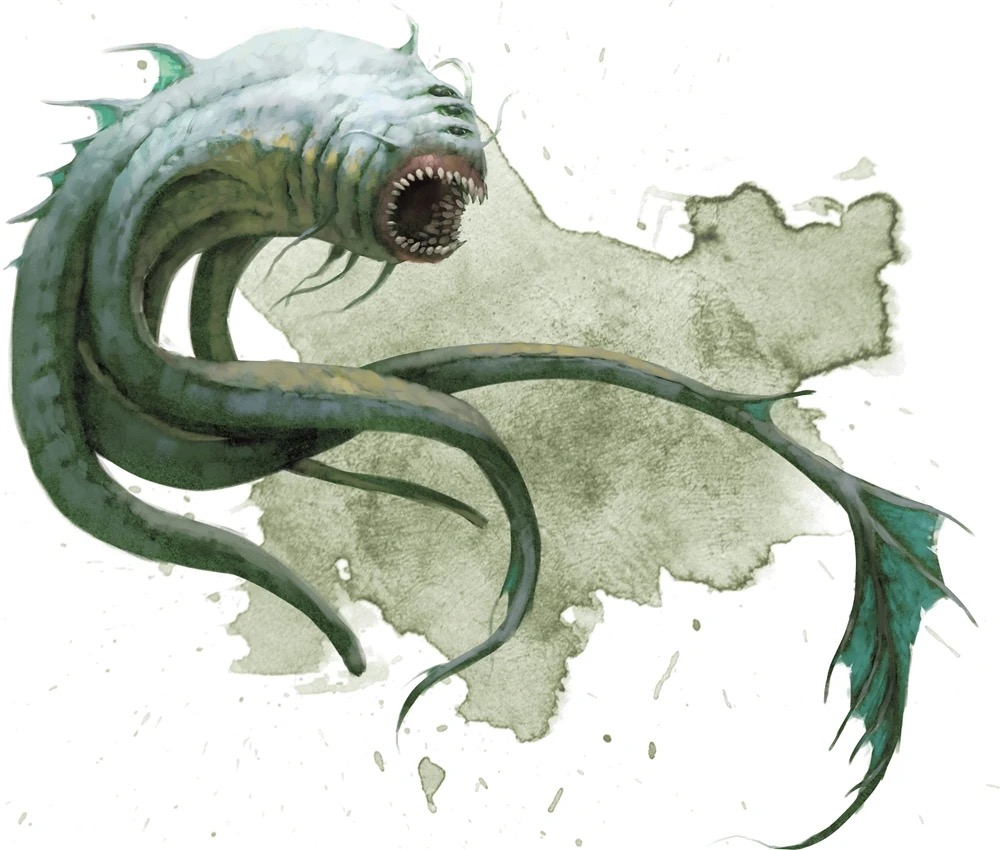
\includegraphics{ABOLETH.webp}
\caption{ABOLETH.webp}
\end{figure}

L'Aboleth riesce a infettare i protettori con i suoi tentacoli e, con i
suoi poteri psichici, riesce a controllare la mente di Gario, che si
scaglia contro i suoi compagni. Lo scontro è estenuante, riducendo Borh
al limite della vita, ma alla fine è proprio lui che riesce ad abbattere
la bestia, liberando Gario dal suo controllo. Gario cura se stesso e i
suoi compagni, che sono stati contaminati dall'Aboleth. I protettori
capiscono in fretta che i conigli sono fuggiti nelle foreste di Drakonia
a causa dell'arrivo dell'Aboleth e che non possono più far nulla.
Tornano quindi ad Azura con i cinque conigli catturati, tre vivi e due
morti (ma non decomposti grazie ai poteri magici di Gario). Al loro
ritorno alla Gilda, vengono nuovamente accolti da Sithau e Jianico.
Gario racconta tutto ciò che è accaduto a Sithau. Sithau appare calmo,
mentre lo chef Jianico è visibilmente alterato alla vista di soli cinque
conigli. Sithau fa uscire lo chef dal suo ufficio con prepotenza, e gli
consegna i cinque conigli, poi chiude la porta e si siede. Sithau,
furioso, sbraita e addirittura spacca la sua scrivania a metà con un
pugno. I protettori hanno violato il codice della gilda, essendo stati
avvertiti di non oltrepassare i confini di Drakonia e soprattutto di non
attaccare le guardie di confine. Sithau e i protettori saranno tutti
sottoposti ad un processo.

Il Processo sarà presieduto dal Gran Consiglio della Gilda. C'è il
timore che, in caso di scoppio di una guerra con Drakonia, i protettori
(e forse anche Sithau) vengano considerati direttamente colpevoli e
possano essere incarcerati o addirittura subire conseguenze peggiori.
Fino al termine del processo, ai protettori vengono confiscate armi e
distintivo, inoltre non è permesso partecipare a missioni o allontanarsi
dalla gilda di Azura.
